\begin{figure}[t]

\begin{minipage}[t]{\linewidth}

{\centering 

\begin{Shaded}
\begin{Highlighting}[]
\ImportTok{import}\NormalTok{ numpy }\ImportTok{as}\NormalTok{ np}
\ImportTok{from}\NormalTok{ poincare }\ImportTok{import}\NormalTok{ Simulator}

\NormalTok{sim }\OperatorTok{=}\NormalTok{ Simulator(Oscillator)}
\NormalTok{df }\OperatorTok{=}\NormalTok{ sim.solve(save\_at}\OperatorTok{=}\NormalTok{np.linspace(}\DecValTok{0}\NormalTok{, }\DecValTok{5}\NormalTok{, }\DecValTok{101}\NormalTok{))}
\end{Highlighting}
\end{Shaded}

}

\end{minipage}%
\newline
\begin{minipage}[t]{0.45\linewidth}

{\centering 

\begin{Shaded}
\begin{Highlighting}[]
\NormalTok{df.head()}
\end{Highlighting}
\end{Shaded}

\begin{longtable}[]{@{}lll@{}}
\toprule\noalign{}
& x & v \\
time & & \\
\midrule\noalign{}
\endhead
\bottomrule\noalign{}
\endlastfoot
0.00 & 1.000000 & 0.000000 \\
0.05 & 0.998750 & -0.049979 \\
0.10 & 0.995005 & -0.099835 \\
0.15 & 0.988772 & -0.149440 \\
0.20 & 0.980069 & -0.198672 \\
\end{longtable}

}

\end{minipage}%
\hfill
\begin{minipage}[t]{0.45\linewidth}

{\centering 

\begin{Shaded}
\begin{Highlighting}[]
\NormalTok{df.plot()}\OperatorTok{;}
\end{Highlighting}
\end{Shaded}

\begin{figure}[H]

{\centering 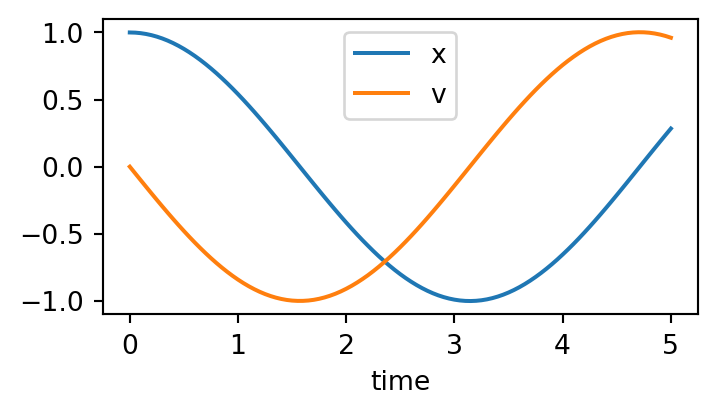
\includegraphics{article_files/figure-latex/cell-9-output-1.pdf}

}

\end{figure}

}

\end{minipage}%

\caption{\label{fig-sim}Simulation of the \texttt{Oscillator} system
from Figure~\ref{fig-second-order}. The output is a
\texttt{pandas.DataFrame} with a column for each variable and the time
as index. It is inspected and plotted with the \texttt{pandas} methods.}

\end{figure}
